\section{纹理坐标函数}
纹理映射的关键是,建立一个世界坐标$(x,y,z)$至纹理坐标$(u,v)$的映射$\phi$
\begin{Equation}
    \phi: (x,y,z)\to(u,v)
\end{Equation}
该函数称为纹理坐标函数(Texture Coordinate Function),其中通常取$(u,v)\in[0,1]^2$。有趣的是,尽管常说“贴图”,但我们实际需要的却是反向的过程:对于模型上给定的一点,找到纹理上的对应点。当然,我们固然可以使用任何函数作为$\phi$,但最好能考虑以下几条性质
\begin{itemize}
    \item 双射性(Bijectivity):物体表面上的点和贴图上的点是一一对应的。
    \item 大小失真(Size Distortion),物体表面上等距分布的点在贴图上仍应当是等距分布。
    \item 形状失真(Shape Distortion),物体表面上的圆在贴图上仍应当大致是圆。
    \item 连续性(Continuity),物体表面上的邻近点在贴图上仍应当是邻近点。
\end{itemize}
没有一个最正确的纹理坐标函数,我们需要根据模型的形状选择最合适的纹理坐标函数。

\begin{Figure}[纹理贴图]
    \begin{FigureSub}[草方块]
        
\includegraphics[width=5cm]{image/Texture/GrassIM.png}
    \end{FigureSub}
    \hspace{1cm}
    \begin{FigureSub}[土方块]
        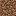
\includegraphics[width=5cm]{image/Texture/DirtIM.png}
    \end{FigureSub}
\end{Figure}

\subsection{平面投影}
平面投影(Planar Projection)是最简单的投影方式。它基本上就是把$(x,y,z)$中的$(x,y)$照抄到$(u,v)$上。试想,若需要纹理贴图的模型本身就是一个平面,这种投影方式将工作的很好。本节暂且假定$(x,y,z)\in[-1,1]^3$,因此对于$x,y$平面上的的平面投影,可以写作
\begin{BoxFormula}[平面投影]
    平面投影可以表达为
    \begin{Gather}[6pt]
        u=\frac{1}{2}(1+x)\\
        v=\frac{1}{2}(1+y)
    \end{Gather}
\end{BoxFormula}

\xref{fig:平面投影}展示了平面投影在球上的效果,前后两个半球分别被两张贴图覆盖。但注意到,在两个半球的交界处的纹理显得有些怪异,图案被拉长。这是因为交界处的$x,y$几乎不变化的缘故。
\begin{Figure}[平面投影]
    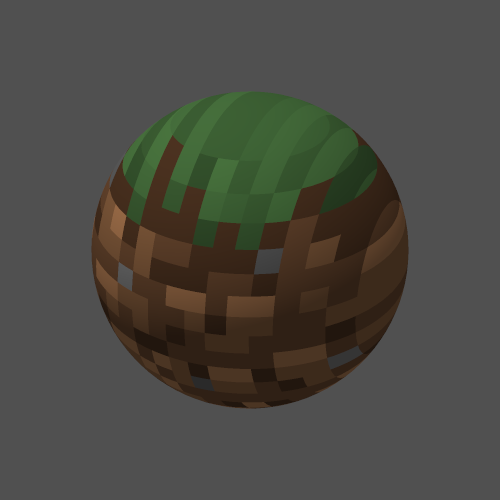
\includegraphics[width=6.5cm]{image/RasterizationIOW/TexPlaner.png}
\end{Figure}

平面投影其实并不一定局限在和坐标轴平齐的方向上,也可以在任意角度进行,还可以带有透视。只需复用\xref{chap:视角变换}视角变换中的正交投影或透视投影的变换矩阵即可,这里不再赘述。

\subsection{球面投影}
球面投影(Spherical Projection)的$u,v$由方位角$\phi\in[-\pi,\pi]$和天顶角$\theta\in[0,\pi]$构成,两者相当于经度(Longtitude)和纬度(Lantitude)。考虑到最终$(u,v)\in[0,1]^2$,变换可以写为
\begin{BoxFormula}[球面投影]
    \begin{Gather}[6pt]
        u=\frac{1}{2\pi}\qty[\pi+\atantwo(y,x)]\\
        v=\frac{1}{\pi}\qty[\pi-\acos(z/|x|)]
    \end{Gather}
\end{BoxFormula}

这里$\atantwo(y,x)$基本上就是$\atan(y/x)$,但做了些处理保证连续性
\begin{Equation}
    \atantwo(y,x)=\begin{cases}
        \atan(y/x),&x>0\\
        \atan(y/x)+\pi,&x<0, y\geq 0\\
        \atan(y/x)-\pi,&x<0, y< 0\\
        +\pi/2,&x=0, y>0\\
        -\pi/2,&x=0, y<0\\
        \text{undefined},&x=0, y=0
    \end{cases}
\end{Equation}

\xref{fig:球面投影}展示了球面投影在球上的效果,可以预见,效果相当不错。
\begin{Figure}[球面投影]
    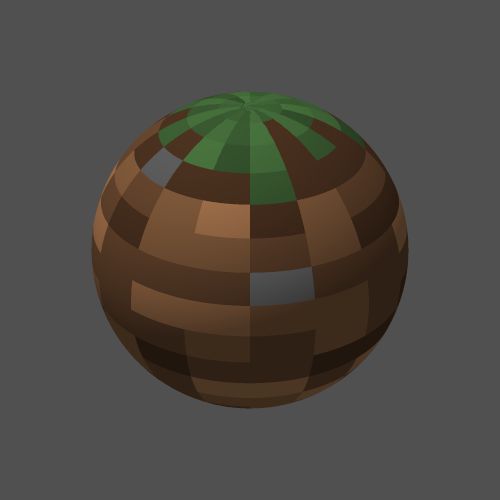
\includegraphics[width=6.5cm]{image/RasterizationIOW/TexSpherical.png}
\end{Figure}

\subsection{柱面投影}
柱面投影(Cylinidrical Projection)的$u,v$由方位角$\phi\in[-\pi,\pi]$和高度$z$构成。
\begin{BoxFormula}[柱面投影]
    \begin{Gather}[6pt]
        u=\frac{1}{2\pi}\qty[\pi+\atantwo(y,x)]\\
        v=\frac{1}{\pi}\qty[1+z]
    \end{Gather}
\end{BoxFormula}

\xref{fig:球面投影}展示了柱面投影在球上的效果,可以看出,柱面投影和球面投影在这个例子中的差别并不大。然而,柱面投影随着靠近南北极,图案会逐渐被拉长,球面投影在该过程中是等长的。
\begin{Figure}[柱面投影]
    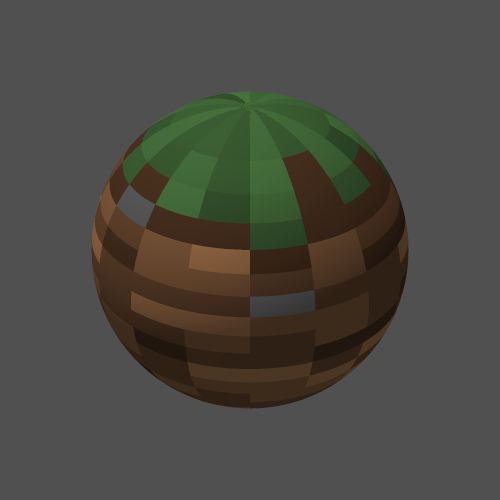
\includegraphics[width=6.5cm]{image/RasterizationIOW/TexCylindrical.png}
\end{Figure}

\subsection{立方体投影}
立方体投影(Cubemap Projection)是对\xref{subsec:平面投影}的平面投影的推广,我们将六个面分别映射到六张纹理上。这里会采用透视投影,故投影至垂直于$z$轴的面的方程就应当是
\begin{Equation}
    u=\frac{x}{z}\qquad v=\frac{y}{z}
\end{Equation}
然而,一个容易混淆的问题是,在六个面上$u,v$的方向按照何种规范定义?关于这一问题有约定俗成的标准,其会保证从内部看$v$位于$u$的逆时针。在这一规范下,变换可以写为
\begin{BoxFormula}
    立方体投影可以表示为
    \begin{Gather}[6pt]
        \phi_{-x}(x,y,z)=\frac{1}{2}[1+(+z,-y)/|x|],\quad |x|>|y|,|z|,\quad x<0\\
        \phi_{+x}(x,y,z)=\frac{1}{2}[1+(-z,-y)/|x|],\quad |x|>|y|,|z|,\quad x>0\\
        \phi_{-y}(x,y,z)=\frac{1}{2}[1+(+x,-z)/|y|],\quad |y|>|z|,|x|,\quad y<0\\
        \phi_{+y}(x,y,z)=\frac{1}{2}[1+(+x,+z)/|y|],\quad |y|>|z|,|x|,\quad y>0\\
        \phi_{-z}(x,y,z)=\frac{1}{2}[1+(-x,-y)/|z|],\quad |z|>|x|,|y|,\quad z<0\\
        \phi_{+z}(x,y,z)=\frac{1}{2}[1+(+x,-y)/|z|],\quad |z|>|x|,|y|,\quad z>0
    \end{Gather}
\end{BoxFormula}


\xref{fig:立方体投影}展示了立方体投影投影在球上的效果,侧面使用了草方块纹理,顶面使用了泥土纹理。
\begin{Figure}[立方体投影]
    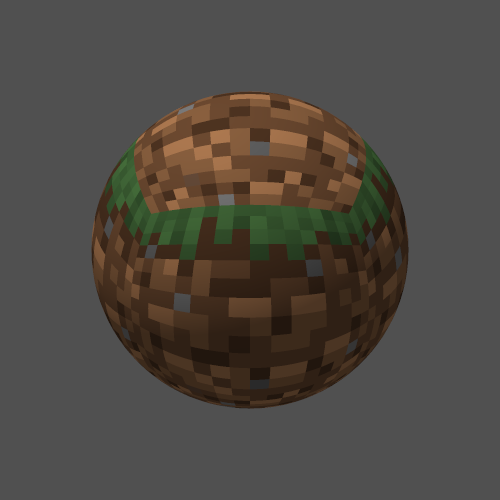
\includegraphics[width=6.5cm]{image/RasterizationIOW/TexCubemap.png}
\end{Figure}
